% \chapter{Wstęp}
\section{Zakres}
	Praca obejmuje implementację sterownika, którego analizę możemy podzielić na:

	\subsection{Baza danych}
	\begin{itemize}
		\item Implementacja:
		\begin{itemize}
			\item \textit{std::vector<std::string, std::any>}
			\item Programowanie optymalne dla cache-u procesora
		\end{itemize}
		\item Klucz:
		\begin{itemize}
			\item Generowanie unikalnego;
			\item Walidacja - Extended \textit{POSIX Regexp}: ,,/[a-z]+\_[1-9]+'';
		\end{itemize}
		\item Operacje:
		\begin{itemize}
			\item Dodaj;
			\item Usuń;
			\item Aktualizuj;
			\item Pobierz wartość na podstawie : konkretnego/typu klucza;
		\end{itemize}
	\end{itemize}
    \begin{figure}[h!]
        \centering
        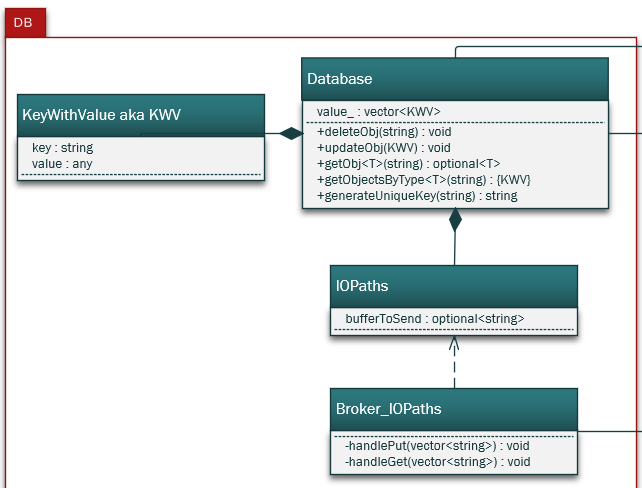
\includegraphics[scale=0.90]{Obrazki/DiagramyKlas/DB.png}
        \caption{Diagram klas przedstawiający relacje klas tworzących bazę danych.
            \newline(Opracowanie własne)}
    \end{figure}

	\subsection{Back-end}
	\begin{itemize}
		\item Realizacja wzorców projektowych:
		\begin{itemize}
			\item Komenda;
			\item Metoda szablonowa;
			\item Obiekt pusty;
			\item Budowniczy;
			\item \textit{RAII};
			\item Wstrzykiwanie zależności;
		\end{itemize}
		\item Implementacja:
		\begin{itemize}
			\item L1 - Warstwy fizycznej;
			\item L2 - Warstwy łącza danych;
			\item L7 - Warstwy aplikacyjnej;
		\end{itemize}
		\item Logowanie ruchu aplikacji:
		\begin{itemize}
			\item <h:min::s::ms> priorytet [nazwaPliku::nazwaFunkcji:numerLinii] komunikat;
			\item Obsługiwane priorytety: Trace < Debug < Info <  Warning < Error
			\item Filtrowanie w zależności od wybranego minimalnego priorytetu
			\item Rezultat przekazywany na wyjście standardowe oraz do pliku tekstowego
		\end{itemize}
	\end{itemize}
